\documentclass[11pt,a4paper]{article}

\usepackage[utf8]{inputenc}
\usepackage[T1]{fontenc}
\usepackage[english]{babel}
\usepackage[a4paper,margin=2.4cm]{geometry}

\usepackage{amsmath, amssymb, amsthm}
\usepackage{mathtools}
\usepackage{booktabs}
\usepackage{tabularx}
\usepackage{array}
\usepackage{caption}
\usepackage{float}
\usepackage{enumitem}
\usepackage{microtype}
\usepackage{xcolor}
\usepackage{listings}
\usepackage{fancyhdr}
\usepackage{titlesec}
\usepackage{graphicx}
\usepackage{adjustbox}
\usepackage{tikz}
\usetikzlibrary{positioning, arrows.meta, fit, backgrounds, calc, shapes.geometric,
                decorations.pathreplacing}
\usepackage[hidelinks]{hyperref}

%  ---  Palette shared with the companion reports  ---
\definecolor{ink}{RGB}{26,30,36}
\definecolor{slate}{RGB}{92,101,112}
\definecolor{mist}{RGB}{233,235,238}
\definecolor{rulegrey}{RGB}{188,194,201}
\definecolor{steel}{RGB}{47,72,102}
\definecolor{steellight}{RGB}{124,146,172}
\definecolor{signal}{RGB}{160,32,45}

\hypersetup{
    colorlinks=true,
    linkcolor=steel,
    citecolor=steel,
    urlcolor=steel,
    pdftitle={Dividing the Cost: Saturated Cost Partitioning over Pattern Databases},
    pdfauthor={Haniel Ulises},
}

\color{ink}

\setlength{\headheight}{22pt}
\pagestyle{fancy}
\fancyhf{}
\fancyhead[L]{\small\textcolor{slate}{\itshape Dividing the Cost}}
\fancyhead[R]{\small\textcolor{slate}{\thepage}}
\renewcommand{\headrulewidth}{0.4pt}
\renewcommand{\headrule}{\hbox to\headwidth{\color{rulegrey}\leaders\hrule height \headrulewidth\hfill}}

\titleformat{\section}{\normalfont\large\bfseries\color{ink}}{\thesection}{0.7em}{}
\titleformat{\subsection}{\normalfont\normalsize\bfseries\color{ink}}{\thesubsection}{0.7em}{}
\titleformat{\paragraph}[runin]{\normalfont\bfseries\color{slate}}{}{0em}{}[.]

\captionsetup{font=small, labelfont={bf,color=slate}, textfont=footnotesize}

\theoremstyle{definition}
\newtheorem{definition}{Definition}
\newtheorem{proposition}{Proposition}
\newtheorem{remark}{Remark}

\lstdefinestyle{sys}{
    backgroundcolor=\color{mist},
    basicstyle=\ttfamily\scriptsize\color{ink},
    keywordstyle=\color{steel}\bfseries,
    commentstyle=\color{slate}\itshape,
    stringstyle=\color{slate},
    morecomment=[l]{\#},
    morekeywords={class,const,double,inline,return,static,struct,std,for,if},
    frame=single,
    rulecolor=\color{rulegrey},
    framesep=5pt,
    xleftmargin=6pt,
    xrightmargin=0pt,
    breaklines=true,
    showstringspaces=false,
    columns=fullflexible,
    captionpos=b,
}
\lstset{style=sys}

%  ---  Notation  ---
\newcommand{\Task}{\mathcal{T}}
\newcommand{\Prop}{P}
\newcommand{\Act}{A}
\newcommand{\hstar}{h^{*}}
\newcommand{\scf}{\mathrm{scf}}
\newcommand{\pre}{\mathrm{pre}}
\newcommand{\add}{\mathrm{add}}
\newcommand{\del}{\mathrm{del}}
\newcommand{\proj}{\mathrm{proj}}
\newcommand{\code}[1]{\texttt{\small #1}}

\begin{document}

\begin{titlepage}
\centering
\vspace*{2.4cm}
{\color{rulegrey}\rule{\textwidth}{0.8pt}}\\[0.9cm]
{\LARGE\bfseries Dividing the Cost\par}
\vspace{0.5cm}
{\large\color{slate} Saturated Cost Partitioning over Pattern Databases,\\ and the Order That Decides What It Is Worth\par}
\vspace{0.7cm}
{\color{rulegrey}\rule{\textwidth}{0.8pt}}\\[1.4cm]

{\large Haniel Ulises\par}
\vspace{0.3cm}
{\color{slate} Automatic Discovery of Planning Heuristics}\\
\vspace{0.15cm}
{\color{slate}\today}

\vfill
{\color{slate}\small
The framework had reached a point where every admissible component it owned
was priced by a cost function, the check that a set of cost functions is a
legal partition was written, and nothing produced the shares. The maximum over
the components stood as the control, and the question left open was whether a
partition of the same components beats it.

\vspace{0.6em}
It does, and not in the form first implemented. A saturated chain under a fixed
order ties the maximum on mean informedness over the four seven-block instances
and expands fifty per cent more nodes than it, because a component that has
reached its own abstract goal still takes the cost the next component needed.
The maximum over the cyclic rotations of that order is provably at least the
maximum over the components at every state, and measures $0.420$ informedness
against $0.339$ and $13\,084$ expansions against $18\,341$.

\vspace{0.6em}
A third construction puts the two kinds of component under one partition: the
databases saturate, and the landmark bound is priced with what they did not
spend. It dominates both controls by construction and improves on the better of
them by two per cent, which is the least interesting number here and the most
informative. The databases consume seventy to seventy-nine per cent of the cost
mass and convert it into a better bound at twenty-one per cent of the states.
Where the mass goes, and not whether the sum is legal, is what the next
iteration has to decide.}
\vspace{1.2cm}
\end{titlepage}

\tableofcontents
\newpage

%  ======================================================================
\section{Scope}
\label{sec:scope}

Section 6 of the project README establishes two admissible components and one
control. The components are a landmark bound priced by the uniform cost
partition over landmarks, and a set of pattern databases over patterns grown by
bounded causal closure from each goal condition. The control is the maximum
over the databases, which is admissible because a maximum of admissible
heuristics is, and which the README states plainly as the thing a partition has
to beat.

Section 6.4 states why the hypothesis class of the project cannot supply that
partition. Giving component $i$ the cost function $w_i \cdot c$ for weights on
the simplex is admissible, and the resulting sum is a convex combination of the
components, so it is bounded pointwise by their maximum, which is itself
admissible. A partition of that shape can never beat the control, and there is
nothing in it to discover. Only the general form, in which each component
receives its own cost function over actions, can exceed the maximum, and it
does so exactly because the cost mass the components charge for is disjoint.

This report closes that gap. It states the construction and proves what it
gives, records two facts about the existing code that had to change before the
construction could be written, reports the measurement on the same instances
and against the same controls the README already uses, and states one negative
result that the first implementation produced and that survives into the
design.

Four claims are established, and are stated narrowly.

\begin{enumerate}[itemsep=3pt, topsep=4pt]
  \item A pattern database has a least cost function preserving its whole
        table, computable from the abstract transition relation it already
        enumerates, and a chain of databases each built under what its
        predecessors left spends the task's costs exactly once.
  \item The sum over such a chain is admissible and consistent, and it is
        \emph{not} in general at least the maximum over the same components.
        A witness is exhibited, and it is a state of one of the unit test
        fixtures.
  \item The maximum over the cyclic rotations of the chain is at least the
        maximum over the components at every state, by an argument that does
        not depend on the patterns, the domain, or the number of components.
        On the four seven-block instances it improves mean informedness from
        $0.339$ to $0.420$ and reduces A\textsuperscript{*} expansions from
        $18\,341$ to $13\,084$.
  \item A partition across component kinds, in which the databases saturate
        and the landmark bound is priced with the remainder, dominates both
        controls by construction. Its measured improvement over the better
        control is two per cent, and the reason is measurable: the databases
        take most of the cost mass and use it at a minority of the states.
\end{enumerate}

What is not established is the ceiling. Optimal cost partitioning, computed per
state by linear programming, is the standard reference point for how much of
the available bound a scheme recovers, and it is not implemented here. Every
number below is therefore a comparison against the controls of section 6 and
not against the best a partition of these components could do.

%  ======================================================================
\section{What existed before, and the two things that did not}
\label{sec:before}

The engine already took cost functions everywhere they were needed. The type
\code{ActionCosts} carries one cost per action of a task and refuses anything
negative, infinite, or not a number, because a negative cost breaks both
admissibility and the Dijkstra that computes $\hstar$, and a silent
\code{NaN} propagates through both. \code{LandmarkFactory} prices landmarks
with a supplied instance of it, \code{PatternDatabase} is built under one,
\code{enumerate\_state\_space} computes $\hstar$ under one, and
\code{is\_cost\_partition} checks that the shares of an action never exceed
what the action costs in the task. A component could therefore be checked
against the goal distances of the same task under the same costs it was
evaluated with, which is the property that makes a partition verifiable rather
than merely asserted.

Two things were missing, and both were invisible until saturation needed them.

\subsection{A projection forgets which actions it kept}
\label{sec:origin}

Projecting a task onto a pattern drops every action that neither adds nor
deletes anything inside the pattern. Such an action is a self-loop in the
abstraction: it cannot shorten an abstract distance, and keeping it multiplies
the transitions to enumerate for nothing. The consequence is that the action
indices of the abstract task are not those of the concrete one.

Nothing depended on that until now, because a database was only ever read. A
saturated cost function is computed over abstract transitions and has to be
returned to the task, so an abstract action index has to be translatable back.
The projection now carries the map.

\begin{lstlisting}
struct Projection {
  StripsTask task;
  ActionCosts costs;
  // Which action of the original task each kept action came from.
  std::vector<std::size_t> origin;
};
\end{lstlisting}

The test that keeps it honest is the same one that documents the drop: in the
two-switch fixture the projection onto $\{\code{off\_x}, \code{on\_x}\}$ keeps
one of the two actions, and \code{origin[0]} is the index of \code{flip\_x} in
the task.

\subsection{The test for keeping an action is needed before any database exists}
\label{sec:touches}

The condition under which a projection keeps an action was written inside the
projection loop. A cost partition has to decide which components can use an
action \emph{before} any of them is built, because the uniform scheme divides
an action's cost among exactly those components. The predicate is now named,
and \code{project} calls it, so the two cannot drift apart:

\begin{lstlisting}
inline bool touches(const StripsAction& action, const StripsState& pattern) {
  return action.add.count_common(pattern) > 0 || action.del.count_common(pattern) > 0;
}
\end{lstlisting}

\subsection{A landmark set does not depend on what it is paid}
\label{sec:value-under}

Which propositions are landmarks of a state is a question about relaxed
reachability, and costs do not enter it. The pricing is one pass over the
actions. The factory computed both together and exposed only the total under
the costs it was constructed with, so serving several shares of a partition
meant several factories and several generations of the same set. The pricing is
now a separate entry point, \code{value\_under(costs, s)}, and \code{value(s)}
calls it with the factory's own costs. Generation is still cached against the
state it was asked about, so one factory answers $k+1$ shares at one state for
the cost of one generation. This matters in section~\ref{sec:mixed}, where
exactly that happens.

%  ======================================================================
\section{The construction}
\label{sec:construction}

\subsection{Cost partitions}

\begin{definition}[Cost partition]
Let $\Task = \langle \Prop, \Act, s_0, G \rangle$ be a planning task with cost
function $c : \Act \to \mathbb{R}_{\ge 0}$. A tuple $\langle c_1, \dots, c_k
\rangle$ of cost functions is a \emph{cost partition} of $c$ when
\[
  c_i(a) \;\ge\; 0 \quad\text{for every } i \text{ and } a,
  \qquad
  \sum_{i=1}^{k} c_i(a) \;\le\; c(a) \quad\text{for every } a \in \Act .
\]
\end{definition}

Costs may be left unspent, and only overspending breaks the bound. That is why
the check tests one inequality per action and not an equality.

\begin{proposition}[The sum under a partition is a bound]
\label{prop:partition}
Let $h_1, \dots, h_k$ be admissible for $\Task$ under $c_1, \dots, c_k$
respectively, where $\langle c_1, \dots, c_k \rangle$ is a cost partition of
$c$. Then $\sum_i h_i$ is admissible for $\Task$ under $c$.
\end{proposition}

\begin{proof}
Let $\pi = \langle a_1, \dots, a_m \rangle$ be an optimal plan from $s$, of
cost $\hstar(s) = \sum_j c(a_j)$. Each $h_i$ is admissible under $c_i$, and
$\pi$ is a plan under every cost function, so $h_i(s) \le \sum_j c_i(a_j)$.
Summing over $i$ and exchanging the order of summation,
\[
  \sum_{i} h_i(s) \;\le\; \sum_{j} \sum_{i} c_i(a_j)
                  \;\le\; \sum_{j} c(a_j) \;=\; \hstar(s). \qedhere
\]
\end{proof}

The proof uses nothing about the components except that each is a bound under
its own share. It holds for components of different kinds, which is what
section~\ref{sec:mixed} relies on, and it holds when the shares are chosen per
state, which is what makes optimal cost partitioning by linear programming
well defined even though it is not implemented here.

\subsection{Saturation}

A pattern database stores the exact goal distance of every abstract state under
the costs it was built with. Reading a table computed under one cost function
while charging for another is only sound if the table survives the change.

\begin{definition}[Saturated cost function]
Let $D$ be a pattern database over pattern $\Prop_i$, built under costs $c$,
with abstract goal distances $h_i$. Its \emph{saturated cost function} is
\begin{gather*}
  \scf_i(a) \;=\; \min\bigl(\, c(a),\; \delta_i(a) \,\bigr),
  \qquad
  \delta_i(a) \;=\; \max\Bigl( \{\, 0 \,\} \cup D_i(a) \Bigr), \\[2pt]
  D_i(a) \;=\;
  \bigl\{\, h_i(u) - h_i(v) \;\bigm|\;
     u \xrightarrow{\ \proj(a)\ } v \text{ in the abstraction},\;
     h_i(u), h_i(v) < \infty \,\bigr\},
\end{gather*}
where $\scf_i(a) = 0$ for every action the projection drops.
\end{definition}

Two families of transition are excluded and the exclusions are not cosmetic.
A transition leaving a dead end has $h_i(u) = \infty$, no search will expand
such a state, and the difference is undefined. A transition entering a dead end
has $h_i(v) = \infty$, so $h_i(u) - h_i(v)$ is negative without bound and the
requirement below is met by every non-negative number. Charging for either
takes cost away from the components that come after this one and buys nothing
here. The first implementation charged the whole of $h_i(u)$ for a transition
into a dead end, which is admissible and wasteful; it is recorded in
section~\ref{sec:defects}.

\begin{proposition}[A database keeps its table under its saturated costs]
\label{prop:saturate}
$h_i$ is admissible for the projected task under $\scf_i$.
\end{proposition}

\begin{proof}
Every abstract goal state has $h_i = 0$, so $h_i$ is goal aware. For every
abstract transition $u \xrightarrow{\ \proj(a)\ } v$ with both distances
finite, the definition gives $\scf_i(a) \ge h_i(u) - h_i(v)$, hence
$h_i(u) \le \scf_i(a) + h_i(v)$; when $h_i(v) = \infty$ the inequality holds
for any finite left-hand side. So $h_i$ is consistent under $\scf_i$.

Let $s$ be a state with a finite goal distance under $\scf_i$ and let
$\langle a_1, \dots, a_m \rangle$ be an optimal $\scf_i$-plan from $s$ through
states $s = u_0, \dots, u_m$ with $u_m$ a goal state. Every $u_j$ lies on a
path to a goal, so every $h_i(u_j)$ is finite. Telescoping consistency along
the path,
\[
  h_i(s) \;\le\; \scf_i(a_1) + h_i(u_1) \;\le\; \cdots
         \;\le\; \sum_{j=1}^{m} \scf_i(a_j) + h_i(u_m)
         \;=\; \hstar_{\scf_i}(s). \qedhere
\]
\end{proof}

The clip at $c(a)$ is what makes the result a share and not a demand. A drop
larger than the action's own cost is possible, because the projection can fold
several concrete actions into one abstract action; taking the drop unclipped
would let one component charge more than the task ever pays.

\begin{figure}[H]
\centering
\begin{adjustbox}{max width=\linewidth}
\begin{tikzpicture}[font=\footnotesize, >={Latex[length=4pt]}]
  \node[anchor=west,align=left,steel] at (0, 1.55)
       {$c_i(a) \;=\; \displaystyle\max_{\,u \xrightarrow{\,a\,} v\,}
        \bigl( h_i(u) - h_i(v) \bigr)$,
        clipped to $[\,0,\ \text{what component } i \text{ was given}\,]$};
  \node[anchor=east] at (-0.15, 0.4) {$c(a)$};
  \fill[steel!12] (0,0) rectangle (5.4,0.8);
  \draw[steel,thick] (0,0) rectangle (2.8,0.8);
  \draw[steel,thick] (2.8,0) rectangle (4.6,0.8);
  \draw[steel,thick] (4.6,0) rectangle (5.4,0.8);
  \draw[slate,thick] (5.4,0) rectangle (8.0,0.8);
  \node[steel] at (1.4,0.4) {$c_1(a)$};
  \node[steel] at (3.7,0.4) {$c_2(a)$};
  \node[steel,font=\scriptsize] at (5.0,0.4) {$c_3$};
  \node[slate] at (6.7,0.4) {leftover};
  \draw[decorate,decoration={brace,amplitude=4pt,mirror},steel] (0,-0.15) -- (5.4,-0.15);
  \draw[decorate,decoration={brace,amplitude=4pt,mirror},slate] (5.4,-0.15) -- (8.0,-0.15);
  \node[steel,anchor=north] at (2.7,-0.42) {taken by the databases, in order};
  \node[slate,anchor=north] at (6.0,-1.02) {left for a component of another kind};

  \node[anchor=east] at (-0.15,-2.05) {uniform};
  \draw[signal,thick,fill=signal!8] (0,-2.35) rectangle (2.0,-1.75);
  \draw[signal,thick,fill=signal!8] (2.0,-2.35) rectangle (4.0,-1.75);
  \draw[signal,thick,fill=signal!8] (4.0,-2.35) rectangle (6.0,-1.75);
  \node[signal] at (1.0,-2.05) {$c(a)/k$};
  \node[signal] at (3.0,-2.05) {$c(a)/k$};
  \node[signal] at (5.0,-2.05) {$c(a)/k$};
  \node[anchor=west,signal] at (6.2,-2.05) {every component underpaid};

  \node[anchor=east] at (-0.15,-3.05) {scaled};
  \draw[signal,thick,fill=signal!8] (0,-3.35) rectangle (6.0,-2.75);
  \node[signal] at (3.0,-3.05) {$w\,c(a)$, for every action};
  \node[anchor=west,signal,align=left] at (6.2,-3.05)
       {a convex combination, bounded\\by the maximum of the components};
\end{tikzpicture}
\end{adjustbox}
\caption{One action's cost, divided three ways. The saturated chain gives each
component the least it needs to keep its own table and passes on the rest. The
uniform scheme divides the cost without asking what any component can use. The
scaled scheme is the hypothesis class of section 2.2 of the README, and its
sum is a convex combination of the components, so it cannot exceed their
maximum.}
\label{fig:saturation}
\end{figure}

\subsection{The chain, and what it leaves}

\begin{definition}[Saturated chain]
Given an ordered sequence of patterns $\Prop_1, \dots, \Prop_k$, set $r_0 = c$
and, for $i = 1, \dots, k$, build $D_i$ under $r_{i-1}$, let $c_i = \scf_i$
computed under $r_{i-1}$, and set $r_i = r_{i-1} - c_i$. The heuristic is
$h_{\mathrm{scp}} = \sum_{i} h_i$ and the \emph{leftover} is $r_k$.
\end{definition}

\begin{proposition}[The chain spends the costs exactly once]
\label{prop:chain}
$c_i \ge 0$ for every $i$, $r_k \ge 0$, and
$\sum_{i=1}^{k} c_i(a) + r_k(a) = c(a)$ for every action $a$. In particular
$\langle c_1, \dots, c_k \rangle$ is a cost partition of $c$, and so is
$\langle c_1, \dots, c_k, r_k \rangle$.
\end{proposition}

\begin{proof}
Induction on $i$. The clip in the definition of $\scf$ gives
$0 \le c_i(a) \le r_{i-1}(a)$, so $r_i(a) = r_{i-1}(a) - c_i(a)$ is
non-negative and the subtraction is exact, with no clipping at zero taking
effect. Telescoping, $\sum_{i \le k} c_i(a) = r_0(a) - r_k(a) = c(a) - r_k(a)$.
\end{proof}

Proposition~\ref{prop:saturate} makes each $h_i$ admissible under $c_i$, and
Proposition~\ref{prop:partition} then makes the sum admissible under $c$. The
sum is also consistent, because each component is an abstraction and therefore
consistent under its own share, and a sum of consistent functions is
consistent. This is checked and not assumed: the unit tests verify the shares
against \code{is\_cost\_partition} and the sum against exhaustively enumerated
goal distances on all three fixtures.

%  ======================================================================
\section{The order}
\label{sec:order}

The order is the only free parameter of the chain. Admissibility does not
depend on it, on the patterns, or on the number of components. What does depend
on it is whether the construction is worth anything.

\subsection{A fixed order can lose to the maximum}

\begin{proposition}[No domination]
\label{prop:nodomination}
There is a task, a set of patterns and a state at which
$h_{\mathrm{scp}}(s) < \max_i h_i^{\,c}(s)$, where $h_i^{\,c}$ is component $i$
evaluated under the task's own costs.
\end{proposition}

\begin{proof}
The \code{joint} fixture has propositions $\{\code{start}, \code{left},
\code{right}\}$, goal $\{\code{left}, \code{right}\}$, and three unit-cost
actions: \code{both}, with precondition $\{\code{start}\}$, adding both goal
propositions; \code{take\_left} and \code{take\_right}, adding one each. Causal
closure from each goal condition gives $\Prop_1 = \{\code{start},
\code{left}\}$ and $\Prop_2 = \{\code{start}, \code{right}\}$.

Take $s = \{\code{start}, \code{left}\}$, at which $\hstar(s) = 1$. Under the
task's own costs $D_1$ reports $0$, because its abstract goal $\{\code{left}\}$
is already satisfied at $s$, and $D_2$ reports $1$, because
$\{\code{right}\}$ is not. The maximum over the components is therefore $1$.

In the chain $\langle \Prop_1, \Prop_2 \rangle$, $D_1$ is built under $c$ and
its abstraction contains the transition $\{\code{start}\} \to \{\code{start},
\code{left}\}$ on \code{both}, which drops $h_1$ from $1$ to $0$. So
$\scf_1(\code{both}) = 1$ and $r_1(\code{both}) = 0$. $D_2$ is then built with
\code{both} free, and reaches its abstract goal from $\{\code{start}\}$ at cost
$0$, so $h_2(s) = 0$. At $s$ the chain reports $h_1(s) + h_2(s) = 0 + 0 = 0$,
which is below the maximum of $1$.
\end{proof}

Both values are admissible. Only one of them is informative, and the loss is
not an artefact of a badly chosen pattern: it is the generic behaviour of a
component that has already reached its abstract goal and still saturates
against the actions leading into it.

\begin{figure}[H]
\centering
\begin{adjustbox}{max width=\linewidth}
\begin{tikzpicture}[
    font=\footnotesize, >={Latex[length=4pt]},
    st/.style={rectangle,draw=ink,thick,fill=white,rounded corners=1.5pt,
               minimum height=15pt,inner xsep=4pt},
    gl/.style={st,draw=steel,fill=steel!10},
    hdr/.style={font=\scriptsize\bfseries,color=slate}]

  \node[hdr,anchor=west] at (0, 2.55) {ORDER $\langle P_1, P_2 \rangle$: the sum returns 0};
  \node[hdr,anchor=west] at (0, 1.80) {$P_1 = \{\texttt{start},\texttt{left}\}$};
  \node[gl,anchor=west] (a1) at (0, 1.20) {\texttt{left}};
  \node[anchor=west] at (1.15, 1.20) {$h_1 = 0$, and it takes $c(\texttt{both}) = 1$};
  \node[hdr,anchor=west] at (0, 0.45) {$P_2 = \{\texttt{start},\texttt{right}\}$};
  \node[st,anchor=west] (a2) at (0,-0.15) {\texttt{start}};
  \node[gl,anchor=west] (b2) at (3.30,-0.15) {\texttt{right}};
  \draw[->,signal,thick] (a2) -- node[above,font=\scriptsize,signal,pos=0.5]
        {\texttt{both}, now free} (b2);
  \node[anchor=west,signal] at (4.45,-0.15) {$h_2 = 0$};
  \node[anchor=west,signal] at (0,-1.00)
       {$h_1 + h_2 = 0$, while $\max(1,1) = 1$ and $h^{*} = 1$};

  \begin{scope}[xshift=7.4cm]
  \node[hdr,anchor=west] at (0, 2.55) {ORDER $\langle P_2, P_1 \rangle$: the maximum is recovered};
  \node[hdr,anchor=west] at (0, 1.80) {$P_2 = \{\texttt{start},\texttt{right}\}$};
  \node[st,anchor=west] (a3) at (0, 1.20) {\texttt{start}};
  \node[gl,anchor=west] (b3) at (3.30, 1.20) {\texttt{right}};
  \draw[->,steel,thick] (a3) -- node[above,font=\scriptsize,steel,pos=0.5]
        {\texttt{both}, $c = 1$} (b3);
  \node[anchor=west,steel] at (4.45, 1.20) {$h_2 = 1$};
  \node[hdr,anchor=west] at (0, 0.45) {$P_1 = \{\texttt{start},\texttt{left}\}$};
  \node[gl,anchor=west] (a4) at (0,-0.15) {\texttt{left}};
  \node[anchor=west] at (1.15,-0.15) {$h_1 = 0$, already at its abstract goal};
  \node[anchor=west,steel] at (0,-1.00)
       {$h_2 + h_1 = 1 = h^{*}$, so one rotation is enough};
  \end{scope}
\end{tikzpicture}
\end{adjustbox}
\caption{The witness of Proposition~\ref{prop:nodomination}, and its repair. A
component that has reached its own abstract goal still saturates against the
actions leading into it, and what it takes is what the next component needed.
The rotation in which the starved component leads recovers the loss.}
\label{fig:starvation}
\end{figure}

\subsection{Rotations}

\begin{definition}[Rotated chain]
For patterns $\Prop_1, \dots, \Prop_k$ let $\sigma_i$ be the cyclic rotation
beginning at $\Prop_i$, and let $h^{(i)}$ be the saturated chain under
$\sigma_i$. The heuristic is $h_{\mathrm{rot}} = \max_{i} h^{(i)}$.
\end{definition}

\begin{proposition}[Rotations dominate the maximum]
\label{prop:rotations}
$h_{\mathrm{rot}}(s) \ge \max_i h_i^{\,c}(s)$ at every state $s$, and
$h_{\mathrm{rot}}$ is admissible.
\end{proposition}

\begin{proof}
Admissibility is Proposition~\ref{prop:partition} for each rotation and the
fact that a maximum of admissible functions is admissible. For the domination,
fix $i$. In $\sigma_i$ the component $\Prop_i$ is first, so it is built under
$r_0 = c$ and its table is the one it has on its own, giving $h^{(i)}$ a
summand equal to $h_i^{\,c}(s)$. Every other summand of $h^{(i)}$ is a goal
distance and therefore non-negative, so $h^{(i)}(s) \ge h_i^{\,c}(s)$. Taking
the maximum over $i$ on both sides gives the claim.
\end{proof}

\begin{remark}
This is the smallest family of orders with that property. Dropping rotation $i$
removes the only order in which $\Prop_i$ leads, and the argument no longer
covers the state at which $\Prop_i$ is the maximum. It is not the only family:
any set of permutations in which every component leads at least once will do,
and the rotations are the cheapest such set. Choosing a better one is a search
over permutations, which is the object section~\ref{sec:follows} identifies as
the right thing for this project to discover.
\end{remark}

The cost is $k$ chains of $k$ databases for $k$ goal conditions, paid once
before search. Section~\ref{sec:measure} reports what that is in seconds.

%  ======================================================================
\section{Across kinds: databases and landmarks under one partition}
\label{sec:mixed}

The two components of section 6 are good at different things. The databases are
consistent, cheap to evaluate, and see the interactions inside a pattern. The
landmark bound is better informed and sees facts that every plan needs, at the
price of one relaxed reachability fixpoint per candidate proposition at every
state, and of inconsistency. Taking the maximum of the two discards one of them
at every state. Proposition~\ref{prop:partition} does not require the
components to be of the same kind, so a partition need not.

A landmark bound cannot be saturated the way an abstraction can, and the reason
is structural. An abstraction stores a whole function, so the least cost
function preserving it is a property of the stored table. The landmarks of a
state are recomputed at that state, and there is no stored function to
preserve; the analogue of a saturated cost function would be a different cost
function at every state, which the databases cannot be rebuilt for. So the
chain runs in the only order available: the databases saturate first, and the
landmark bound is priced with the leftover $r_k$, which needs no saturation
because nothing comes after it.

\begin{definition}[Mixed family]
For each rotation $\sigma_i$ let $h^{(i)}$ be its saturated chain over the
databases and $r^{(i)}$ its leftover. Let $h_{\mathrm{LM}}^{\,d}$ denote the
landmark bound priced by cost function $d$. The heuristic is
\[
  h_{\mathrm{mix}}(s) \;=\;
  \max\Bigl(\, h_{\mathrm{LM}}^{\,c}(s),\;
  \max_{i=1..k} \bigl[\, h^{(i)}(s) + h_{\mathrm{LM}}^{\,r^{(i)}}(s) \,\bigr] \Bigr).
\]
\end{definition}

\begin{proposition}[The mixed family dominates both controls]
\label{prop:mixed}
$h_{\mathrm{mix}}$ is admissible, and at every state
$h_{\mathrm{mix}}(s) \ge \max_i h_i^{\,c}(s)$ and
$h_{\mathrm{mix}}(s) \ge h_{\mathrm{LM}}^{\,c}(s)$.
\end{proposition}

\begin{proof}
By Proposition~\ref{prop:chain} the tuple $\langle c_1^{(i)}, \dots,
c_k^{(i)}, r^{(i)} \rangle$ is a cost partition of $c$, so each bracketed sum
is admissible by Proposition~\ref{prop:partition}; the first argument of the
outer maximum is the degenerate partition that gives the landmark bound
everything and the databases nothing, which is admissible as well. A maximum of
admissible functions is admissible.

The second control is dominated because it is one of the members. The first is
dominated by the argument of Proposition~\ref{prop:rotations}: the $i$-th
bracket contains $h^{(i)}(s) \ge h_i^{\,c}(s)$ and a non-negative landmark
term.
\end{proof}

Including the degenerate member is the whole of the second half of that proof,
and it costs one extra pricing of a landmark set that has already been
generated. That is why section~\ref{sec:value-under} separated generation from
pricing: at one state the set is computed once and priced $k+1$ times.

\begin{remark}
$h_{\mathrm{mix}}$ inherits the landmark bound's inconsistency. A\textsuperscript{*}
with an inconsistent heuristic may reopen states, and the measurement in
section~\ref{sec:measure} reports how often that happens. It remains optimal:
reopening is what preserves optimality when consistency fails.
\end{remark}

%  ======================================================================
\section{Implementation}
\label{sec:implementation}

Everything is in headers, and no existing interface changed meaning.

\begin{itemize}[itemsep=3pt, topsep=4pt]
  \item \code{hd/pdb.hpp}. A projection now carries the map back to the
        actions of the task; the test for keeping an action is named
        \code{touches}; and a database computes its saturated cost function at
        construction, from the abstract transitions it already enumerates,
        exposing it and the remainder it leaves. The saturation is one pass
        over the transition relation, so building a database is no more
        expensive than it was.
  \item \code{hd/landmarks.hpp}. \code{value\_under(costs, s)} is the pricing
        pass; \code{value(s)} calls it with the factory's own costs.
  \item \code{hd/heuristic.hpp}. Four new heuristics, one per scheme above:
        the uniform partition, the saturated chain, the rotated family and the
        mixed family. Each exposes the shares it built with, so a test can
        check the partition property against the task instead of trusting the
        construction.
  \item \code{hd/runner.hpp} and the two command line tools. Four new
        specification names, \code{pdb\_uniform} and \code{scp} and
        \code{scp\_rotations} and \code{scp\_mixed}, accepted anywhere a
        heuristic is. Dispatch stays a template, so no virtual call enters the
        evaluation path.
\end{itemize}

The chain itself is three statements, which is the point of having had the
cost plumbing in place first:

\begin{lstlisting}
SaturatedPatternDatabaseHeuristic(const StripsTask& task,
                                  const std::vector<StripsState>& patterns)
    : remaining_(ActionCosts::of(task)) {
  for (const StripsState& pattern : patterns) {
    databases_.emplace_back(task, pattern, remaining_);
    shares_.push_back(databases_.back().saturated_costs());
    remaining_ = databases_.back().remainder(remaining_);
  }
}
\end{lstlisting}

The unit suite went from 87 tests to 104. The seventeen new ones cover the
saturated share being a share, the remainder adding back to what was given, a
database staying admissible when verified against goal distances recomputed
under its own saturated costs, the partition property of every construction,
the witness of Proposition~\ref{prop:nodomination} pinned as an equality so it
cannot be lost, the domination of Proposition~\ref{prop:rotations} at every
state of all three fixtures, and the exact spending of
Proposition~\ref{prop:chain}.

%  ======================================================================
\section{Measurement}
\label{sec:measure}

\subsection{Setup}

The four Blocksworld instances of seven blocks, which are the instances section
6.3 of the README already uses. Each has 98 actions and 7 goal conditions, so
each yields 7 patterns under a budget of 12 propositions, and the rotated
constructions build 49 databases. The reachable state spaces total $263\,958$
states, of which $263\,954$ have a finite non-zero goal distance. Informedness
is the mean of $h/\hstar$ over those states, computed by \code{hd\_verify}
against exact goal distances and without running a search. Expansions are the
total over the four instances of A\textsuperscript{*} run to optimality; every
configuration returns plans of total cost 60, as it must.

Times are separated into two columns because the two constructions here have
very different profiles. \emph{Setup} is what the process spends before the
first node is expanded, which for the abstraction heuristics is the enumeration
of every projection. \emph{Search} is what A\textsuperscript{*} spends. The
README reports only the second; a heuristic whose setup exceeds its own search
by an order of magnitude should not be compared on the second alone.

\subsection{The comparison}

\begin{table}[H]
\centering
\caption{The four seven-block instances, verified over the same $263\,958$
states and searched with A\textsuperscript{*}. Informedness and the minimum of
$h/\hstar$ come from the verifier; expansions, reopenings and search time from
the planner. Every row returns optimal plans of total cost 60.}
\label{tab:comparison}
\small
\begin{adjustbox}{max width=\linewidth}
\begin{tabular}{lrrrrrrl}
\toprule
Heuristic & Informedness & Min $h/\hstar$ & Expanded & Lower $g$ & Search & Setup & Verdict \\
\midrule
\code{goal\_count}      & 0.367 & 0.045 & 15\,451 & 0     & 0.01 s & 0.00 s & adm., cons. \\
\code{relaxed\_layers}  & 0.344 & 0.143 & 28\,689 & 0     & 0.15 s & 0.01 s & adm., cons. \\
\code{pdb}              & 0.339 & 0.111 & 18\,341 & 882   & 0.03 s & 0.24 s & adm., cons. \\
\code{pdb\_uniform}     & 0.195 & 0.026 & 68\,781 & 0     & 0.08 s & 0.25 s & adm., cons. \\
\code{scp}              & 0.339 & 0.000 & 27\,655 & 2\,037 & 0.03 s & 0.22 s & adm., cons. \\
\code{scp\_rotations}   & 0.420 & 0.167 & 13\,084 & 379   & 0.09 s & 1.71 s & adm., cons. \\
\code{landmark\_cost}   & 0.520 & 0.268 & 4\,166  & 378   & 0.48 s & 0.00 s & adm., inconsistent \\
\code{scp\_mixed}       & \textbf{0.530} & 0.268 & \textbf{4\,067} & 324 & 1.06 s & 1.64 s & adm., inconsistent \\
\bottomrule
\end{tabular}
\end{adjustbox}
\end{table}

Four things in that table are worth stating separately.

\paragraph{The uniform partition is not a weak control, it is a bad heuristic}
At $0.195$ informedness and $68\,781$ expansions it is well below the maximum
over the same components and below every other row. Dividing an action's cost
among the components that can see it, without asking what any of them can use,
starves all of them at once. This is the control section 6.4 of the README
called for, and it earns its place by being clearly worse than the maximum: it
shows that being a legal partition is not by itself worth anything.

\paragraph{The fixed order ties on the mean and loses on the search}
\code{scp} and \code{pdb} report the same mean informedness to three decimal
places and differ by fifty per cent in expansions. The minimum column explains
it. \code{scp} reaches $0.000$, which is the behaviour of
Proposition~\ref{prop:nodomination} appearing at scale: at some states the
chain returns zero where the maximum returns something. A mean over states
hides that, and A\textsuperscript{*} does not, because the states where the
bound collapses are the ones it then has to expand.

\paragraph{The rotations improve the bound and cost wall time at both ends}
\code{scp\_rotations} improves informedness by $24\%$ over the maximum and
expansions by $29\%$, with a minimum of $0.167$ against $0.111$, which is the
domination of Proposition~\ref{prop:rotations} visible as a floor. It is also
slower in both places. Setup goes from $0.24$ s to $1.71$ s, a factor of about
seven, which is $k$ and is what building $k$ chains costs. Search goes from
$0.03$ s to $0.09$ s despite expanding $29\%$ fewer nodes, because one
evaluation is now $k^2 = 49$ table lookups instead of $k = 7$. At seven blocks
the whole search is a tenth of a second, so the construction is a loss in wall
time and a gain in the quantity this project optimises. The two diverge here
because the instances are small enough that nothing amortises; the ratio of
expansions to lookups per expansion is what decides it at any other size.

\paragraph{The mixed bound dominates both controls and improves on the better one by two per cent}
$0.530$ against $0.520$, and $4\,067$ expansions against $4\,166$. The
domination is exact and by construction, so the margin cannot be negative; it
can be, and here almost is, zero. Search time doubles, from $0.48$ s to
$1.06$ s, because every evaluation prices the landmark set $k+1$ times on top
of $k^2$ table lookups. That margin is the most informative number in the
table, and section~\ref{sec:anatomy} takes it apart.

\subsection{Per instance}

\begin{table}[H]
\centering
\caption{A\textsuperscript{*} expansions per instance. The ordering is the same
on all four, which is what makes the totals worth quoting.}
\label{tab:perinstance}
\small
\begin{adjustbox}{max width=\linewidth}
\begin{tabular}{lrrrr}
\toprule
Heuristic & \code{blocks-07-00} & \code{blocks-07-01} & \code{blocks-07-02} & \code{blocks-07-03} \\
\midrule
\code{goal\_count}     & 7\,325 & 182 & 7\,364 & 580 \\
\code{relaxed\_layers} & 12\,421 & 664 & 13\,204 & 2\,400 \\
\code{pdb}             & 7\,895 & 761 & 8\,626 & 1\,059 \\
\code{pdb\_uniform}    & 29\,686 & 2\,223 & 29\,213 & 7\,659 \\
\code{scp}             & 10\,851 & 1\,057 & 12\,954 & 2\,793 \\
\code{scp\_rotations}  & 5\,784 & 271 & 6\,540 & 489 \\
\code{landmark\_cost}  & 2\,518 & 53 & 1\,506 & 89 \\
\code{scp\_mixed}      & 2\,465 & 51 & 1\,463 & 88 \\
\bottomrule
\end{tabular}
\end{adjustbox}
\end{table}

\code{scp} is worse than \code{pdb} on all four instances and
\code{scp\_rotations} is better on all four. Neither total depends on one
instance carrying it.

\subsection{Where the mixed bound's value comes from}
\label{sec:anatomy}

The two per cent has a cause, and it is measurable without any search. At every
state with a finite non-zero goal distance, compare the two arguments of the
outer maximum: the landmark bound priced with the whole cost function, against
the best of the $k$ mixed rotations.

\begin{table}[H]
\centering
\caption{Which member of the mixed family attains the maximum, over the
$263\,954$ states of the four instances with a finite non-zero goal distance.}
\label{tab:anatomy}
\small
\begin{adjustbox}{max width=\linewidth}
\begin{tabular}{lrr}
\toprule
Winning member & States & Share \\
\midrule
The landmark bound alone, on the whole cost function & 199\,434 & 75.6\,\% \\
A mixed rotation, databases plus the leftover        & 55\,151  & 20.9\,\% \\
Tied                                                 & 9\,369   & 3.5\,\% \\
\midrule
Mean value, landmark bound alone                     & \multicolumn{2}{r}{8.182} \\
Mean value, best mixed rotation                      & \multicolumn{2}{r}{6.631} \\
\bottomrule
\end{tabular}
\end{adjustbox}
\end{table}

The saturated databases consume between $70.4\%$ and $78.6\%$ of the total cost
mass of an instance, depending on the instance, and turn it into a better bound
at $20.9\%$ of the states. At three states in four the correct decision is to
give the databases nothing, and the mixed heuristic makes that decision only
because the degenerate member is in the family.

This is the finding, and it is about the components and not about the scheme.
Saturation is optimal for one component in isolation: it takes the least cost
that preserves that component's table. It is not optimal for a chain, because
what one component needs to preserve its table is not what it needs to be
useful, and a component that has reached its abstract goal preserves a table of
zeros at full price. The seven goal-condition patterns of a Blocksworld
instance overlap heavily, and each one preserves a great deal that a landmark
bound would have priced better.

%  ======================================================================
\section{Defects and corrections}
\label{sec:defects}

\paragraph{The first saturation charged for transitions into dead ends}
The definition read: skip a transition out of a dead end, and for a transition
into one charge the whole of $h_i(u)$, on the reasoning that an action leading
nowhere cannot help the abstraction and this is the largest drop the transition
could justify. That is admissible, because the clip at $c(a)$ still holds, and
it is wrong as an answer to the question saturation asks. The constraint such a
transition imposes is $\scf_i(a) \ge h_i(u) - \infty$, which every non-negative
number satisfies. The charge was cost taken from later components for nothing.
It is now skipped, and the proof of Proposition~\ref{prop:saturate} is written
so that the case is visible.

\paragraph{The first test asserted a domination that does not hold}
The test written alongside \code{scp} asserted that the sum is never below the
maximum of its own components, with a comment saying that this is not a theorem
in general and holds here because the leading component is the one the maximum
picks. It failed on the \code{joint} fixture on the first run. The comment was
right about the general case and wrong about the fixture, and the failure is
Proposition~\ref{prop:nodomination}. The test is now the counterexample,
pinned as two exact values, and the domination is asserted of
\code{scp\_rotations} instead, where it is a theorem.

\paragraph{The projection dropped actions by inspecting the masked copy}
\code{project} decided whether to keep an action by testing whether the masked
\code{add} and \code{del} were both empty, after masking. That is the same
predicate, but it could only be evaluated after the work of masking had been
done, and the uniform partition needs the answer before any projection exists.
Extracting \code{touches} removed a duplicate of the condition that would have
had to be kept in step by hand.

%  ======================================================================
\section{What the runs establish}
\label{sec:establish}

\begin{enumerate}[itemsep=3pt, topsep=4pt]
  \item A cost partition over the components of section 6 exceeds their
        maximum on the instances of section 6.3, by $24\%$ of informedness and
        $29\%$ of expansions, and the excess is not an artefact of one
        instance.
  \item The general form is necessary and not sufficient. The uniform
        partition is a legal partition of the general form and is the worst
        heuristic measured here, at $0.195$ informedness against $0.339$ for
        the maximum it is supposed to beat.
  \item Saturation alone is not enough either. A single saturated order ties
        the maximum on the mean and is fifty per cent worse in expansions,
        because it collapses to zero at states where a component has already
        reached its abstract goal.
  \item The order is where the value is, and a family of orders that covers
        every component recovers it with a guarantee that holds at every state
        and does not depend on the domain.
  \item A partition across component kinds is admissible, dominates both
        controls by construction, and on these instances is worth two per cent
        over the better of them, because the abstraction components take most
        of the cost mass and are the better bound at a minority of states.
\end{enumerate}

%  ======================================================================
\section{What they do not}
\label{sec:donot}

\paragraph{There is no ceiling in the table}
Optimal cost partitioning, computed per state by a linear program over the
shares, is the reference point that says how much of the available bound a
scheme recovers. Without it, $0.420$ and $0.530$ are comparisons against the
controls and not against what these components could give.

\paragraph{One domain, and small instances}
Everything is Blocksworld, and seven blocks is where exhaustive enumeration is
still cheap. Both constructions here are exponential in the pattern size and
linear in the number of patterns, and the cost of the rotated family is
quadratic in the number of goal conditions, so the wall time reported is a
lower bound on what a larger domain would cost.

\paragraph{Pattern selection is untouched}
The patterns are one per goal condition, grown by bounded causal closure to
twelve propositions. The README already records that raising the budget keeps
improving informedness at seven blocks, which says that pattern selection
matters at least as much as the partition over the patterns. A scheme that
divides costs well among badly chosen components is still limited by the
components.

\paragraph{The rotations are a family and not a choice}
$h_{\mathrm{rot}}$ takes a maximum over $k$ orders because it cannot tell which
one is right. That is a guarantee bought by paying for all of them. A single
order chosen well would cost $1/k$ of the setup and give up the guarantee, and
nothing here says how to choose it.

%  ======================================================================
\section{What follows}
\label{sec:follows}

\begin{enumerate}[itemsep=4pt, topsep=4pt]
  \item \textbf{Optimal cost partitioning by linear programming}, per state,
        as the ceiling. The shares are the variables, one per component and
        action; the constraints are the partition inequalities and, for each
        component, the requirement that its stored table remains a bound.
        Reported alongside the schemes here, it turns every number in
        Table~\ref{tab:comparison} into a fraction of what was available.
  \item \textbf{The order as the object of discovery.} A permutation of the
        components is small, interpretable, and exactly the kind of thing this
        project exists to search over, and section~\ref{sec:anatomy} says that
        it is where the value is. The objective is already available without
        running a search, since informedness against $\hstar$ is computed by
        the verifier. The immediate experiment is whether a searched
        permutation beats the rotations at $1/k$ of their cost.
  \item \textbf{Diversification instead of enumeration.} The rotations are the
        cheapest family in which every component leads once. A set of orders
        chosen to be diverse over the states actually evaluated is the
        standard improvement, and it changes the question from which order is
        best to which set of orders covers the state space.
  \item \textbf{A second domain.} Gripper or Logistics, added as a generator
        beside the Blocksworld one. The claim that the mixed bound is worth
        two per cent is a claim about Blocksworld and about these patterns.
        Whether the databases take three quarters of the cost mass in a domain
        whose goals do not overlap is the first thing worth checking.
\end{enumerate}

%  ======================================================================
\section*{Reproduction}
\addcontentsline{toc}{section}{Reproduction}

\begin{lstlisting}
cmake -S . -B build -DCMAKE_BUILD_TYPE=Release && cmake --build build -j
./build/cpp/tests/hd_tests                      # 104 tests

# informedness against exact goal distances, no search
./build/hd_verify --instance instances/blocksworld/blocks-07-00.task \
                  --instance instances/blocksworld/blocks-07-01.task \
                  --instance instances/blocksworld/blocks-07-02.task \
                  --instance instances/blocksworld/blocks-07-03.task \
                  --heuristic pdb --heuristic pdb_uniform --heuristic scp \
                  --heuristic scp_rotations --heuristic landmark_cost \
                  --heuristic scp_mixed --max-states 1000000

# expansions, with A* run to optimality
./build/hd_plan --instance instances/blocksworld/blocks-07-00.task \
                --search astar --heuristic scp_rotations --max-expansions 0
\end{lstlisting}

Both tools write one self-describing JSON record carrying the build
provenance, the limits, and every measurement quoted above. The engine is
deterministic: tie-breaking in the open list is by insertion order, and the
patterns are a deterministic function of the task and the budget, so a repeated
run returns identical numbers.

\end{document}
